% =====================================================================
%  លំហាត់ ៣.២ — កម្លាំងប្រតិកម្មនៅទ្រនាប់នៃធ្នឹម (Khmer version)
%  Solved by: ពៅ គឹមយ៉ាត (Pov Kimyat) — Science Master Academic
%  Compile with XeLaTeX.
% =====================================================================
\documentclass[12pt,a4paper]{article}

\usepackage{amsmath,amssymb}
\usepackage{fontspec}
\usepackage[a4paper,top=2.4cm,bottom=2.3cm,left=2.2cm,right=2.2cm,headheight=16pt]{geometry}
\usepackage{enumitem}
\usepackage{xcolor}
\usepackage{tikz}
\usetikzlibrary{arrows.meta,patterns,calc}
\usepackage[most]{tcolorbox}
\usepackage{titlesec}
\usepackage{fancyhdr}
\usepackage{array,booktabs,colortbl}

% ---- Fonts ----
\setmainfont{Latin Modern Roman}
\newfontfamily\khmerfont[Script=Khmer]{Noto Serif Khmer}
\usepackage[Latin,Khmer]{ucharclasses}
\setTransitionsFor{Khmer}{\khmerfont}{\rmfamily}
\linespread{1.15}
\XeTeXlinebreaklocale "km"
\XeTeXlinebreakskip=0pt plus 1pt
\setlength{\parindent}{0pt}
\setlength{\parskip}{2pt}

% ---- Colours ----
\definecolor{navy}{HTML}{14325C}
\definecolor{teal}{HTML}{0E7C86}
\definecolor{gold}{HTML}{C9962B}
\definecolor{crimson}{HTML}{B3263A}
\definecolor{forest}{HTML}{2E7D4F}
\definecolor{paper}{HTML}{F5F8FC}
\definecolor{softteal}{HTML}{E6F4F5}
\definecolor{softgold}{HTML}{FBF4E4}
\definecolor{softred}{HTML}{FBECEE}
\definecolor{softgreen}{HTML}{E9F5EE}
\definecolor{inkgray}{HTML}{4A5563}
\definecolor{loadfill}{HTML}{DCE9F7}
\definecolor{loadline}{HTML}{2F6DB5}

% ---- Headings ----
\titleformat{\section}
  {\large\bfseries\color{navy}}
  {\tikz[baseline=(n.base)]\node[fill=teal,text=white,rounded corners=3pt,
     inner sep=3.5pt,minimum width=1.5em](n){\thesection};}
  {0.6em}{}[{\color{gold}\titlerule[1.1pt]}]
\titlespacing*{\section}{0pt}{0.8em}{0.5em}

% ---- Header / footer ----
\pagestyle{fancy}
\fancyhf{}
\fancyhead[L]{\small\color{navy}\textbf{Science Master Academic}}
\fancyhead[R]{\small\color{teal}ស្តាទិច · លំហាត់ ៣.២}
\fancyfoot[C]{\tikz\node[fill=navy,text=white,circle,inner sep=2.5pt,
  minimum size=1.5em,font=\small\bfseries]{\thepage};}
\fancyfoot[R]{\scriptsize\color{inkgray}ពៅ គឹមយ៉ាត}
\renewcommand{\headrulewidth}{0.8pt}
\renewcommand{\headrule}{{\color{gold}\hrule height\headrulewidth width\headwidth}}

% ---- Boxes ----
\tcbset{base/.style={enhanced,breakable,arc=3pt,boxrule=0pt,left=10pt,right=10pt,
  top=6pt,bottom=6pt,fonttitle=\small\bfseries,coltitle=white,before skip=8pt,after skip=8pt}}
\newtcolorbox{problem}{base,colback=paper,colframe=navy,boxrule=1pt,title={លំហាត់ ៣.២},
  attach boxed title to top left={xshift=8pt,yshift=-2mm},
  boxed title style={colback=navy,arc=2pt,boxrule=0pt}}
\newtcolorbox{given}{base,colback=softteal,colframe=teal,borderline west={4pt}{0pt}{teal},
  title={ទិន្នន័យ},attach boxed title to top left={xshift=8pt,yshift=-2mm},
  boxed title style={colback=teal,arc=2pt,boxrule=0pt}}
\newtcolorbox{note}{base,colback=softgold,colframe=gold,borderline west={4pt}{0pt}{gold},
  title={ចំណាំ},attach boxed title to top left={xshift=8pt,yshift=-2mm},
  boxed title style={colback=gold,arc=2pt,boxrule=0pt}}
\newtcolorbox{answer}{base,colback=softred,colframe=crimson,boxrule=1.2pt,title={ចម្លើយ},
  attach boxed title to top center={yshift=-2mm},
  boxed title style={colback=crimson,arc=2pt,boxrule=0pt}}
\newtcolorbox{checkbox}{base,colback=softgreen,colframe=forest,borderline west={4pt}{0pt}{forest},
  title={ផ្ទៀងផ្ទាត់},attach boxed title to top left={xshift=8pt,yshift=-2mm},
  boxed title style={colback=forest,arc=2pt,boxrule=0pt}}

\newcommand{\N}{\,\mathrm{N}}
\newcommand{\m}{\,\mathrm{m}}

% ---- Beam drawing helpers (1 m = \u cm) ----
\def\u{1.2}
\newcommand{\pinsupport}[1]{%
  \fill[inkgray!60] (#1,0) -- ++(-0.22,-0.38) -- ++(0.44,0) -- cycle;
  \draw[inkgray,thick] (#1,0) -- ++(-0.22,-0.38) -- ++(0.44,0) -- cycle;
  \fill[pattern=north east lines,pattern color=inkgray] (#1-0.35,-0.38) rectangle (#1+0.35,-0.5);
  \draw[inkgray] (#1-0.35,-0.38) -- (#1+0.35,-0.38);}
\newcommand{\rollersupport}[1]{%
  \fill[inkgray!60] (#1,-0.19) circle (0.19);
  \draw[inkgray,thick] (#1,-0.19) circle (0.19);
  \fill[pattern=north east lines,pattern color=inkgray] (#1-0.35,-0.38) rectangle (#1+0.35,-0.5);
  \draw[inkgray] (#1-0.35,-0.38) -- (#1+0.35,-0.38);}

\begin{document}

% =====================================================================
%  Title banner
% =====================================================================
\thispagestyle{empty}
\begin{tikzpicture}[remember picture,overlay]
  \fill[navy] (current page.north west) rectangle ([yshift=-5.4cm]current page.north east);
  \fill[teal] ([yshift=-5.4cm]current page.north west) rectangle ([yshift=-5.75cm]current page.north east);
  \fill[gold] ([yshift=-5.75cm]current page.north west) rectangle ([yshift=-5.9cm]current page.north east);
  \node[text=gold,font=\small\bfseries,anchor=north] at ([yshift=-1.1cm]current page.north)
    {SCIENCE MASTER ACADEMIC};
  \node[text=white,font=\huge\bfseries,anchor=north] at ([yshift=-1.8cm]current page.north)
    {កម្លាំងប្រតិកម្មនៅទ្រនាប់នៃធ្នឹម};
  \node[text=white!85!teal,font=\large,anchor=north] at ([yshift=-3.25cm]current page.north)
    {លំហាត់ ៣.២ · បន្ទុកចែកចាយរាងចតុកោណព្នាយ};
  \node[text=white,font=\normalsize,anchor=north] at ([yshift=-4.3cm]current page.north)
    {ដោះស្រាយដោយ \textbf{ពៅ គឹមយ៉ាត}};
\end{tikzpicture}
\vspace*{3.4cm}

\begin{problem}
ចូរកំណត់\textbf{កម្លាំងប្រតិកម្ម}នៅទ្រនាប់ $A$ និង $B$ នៃធ្នឹម
ដែលទទួលបន្ទុកដូចបង្ហាញក្នុងរូប\allowbreak ខាងក្រោម~។

\begin{center}
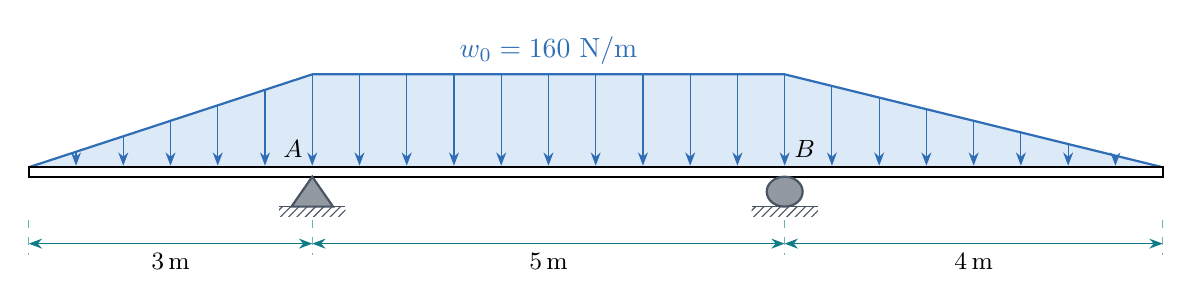
\begin{tikzpicture}[x=\u cm,y=1cm,>=Stealth]
  % load diagram
  \fill[loadfill] (0,0.12) -- (3,1.3) -- (8,1.3) -- (12,0.12) -- cycle;
  \draw[loadline,thick] (0,0.12) -- (3,1.3) -- (8,1.3) -- (12,0.12);
  \foreach \x in {0.5,1,...,11.5}{
    \pgfmathsetmacro{\h}{\x<3 ? 0.12+1.18*\x/3 : (\x<=8 ? 1.3 : 0.12+1.18*(12-\x)/4)}
    \draw[->,loadline] (\x,\h) -- (\x,0.14);}
  \node[above,loadline] at (5.5,1.3) {$w_0 = 160\ \mathrm{N/m}$};
  % beam
  \fill[white] (0,-0.0) rectangle (12,0.12);
  \draw[thick] (0,0) rectangle (12,0.12);
  \pinsupport{3}\rollersupport{8}
  \node[above left] at (3,0.12) {\small$A$};
  \node[above right] at (8,0.12) {\small$B$};
  % dimensions
  \foreach \a/\b/\t in {0/3/3\m,3/8/5\m,8/12/4\m}{
    \draw[<->,teal] (\a,-0.85) -- (\b,-0.85) node[midway,below,text=black]{\small$\t$};}
  \foreach \x in {0,3,8,12} \draw[teal!60,dashed] (\x,-0.55) -- (\x,-1.0);
\end{tikzpicture}
\end{center}
\end{problem}

\begin{given}
\begin{itemize}[leftmargin=1.3em,itemsep=0pt,topsep=0pt]
  \item ធ្នឹមវែង $12\m$ ៖ ផ្នែកលយខាងឆ្វេង $3\m$ ចន្លោះ $AB=5\m$ ផ្នែកលយខាងស្តាំ $4\m$ ។
  \item $A$ ជា\textbf{ទ្រនាប់សន្លាក់} (pin ៖ មានប្រតិកម្ម $A_x$ , $A_y$) ហើយ
        $B$ ជា\textbf{ទ្រនាប់រំកិល} (roller ៖ មានប្រតិកម្ម $B_y$) ។
  \item បន្ទុកកើនជាលីនេអ៊ែរពី $0$ ដល់ $160\ \mathrm{N/m}$ លើផ្នែកលយខាងឆ្វេង
        ស្មើ $160\ \mathrm{N/m}$ ពី $A$ ដល់ $B$ ហើយថយជាលីនេអ៊ែរដល់ $0$
        លើផ្នែកលយខាងស្តាំ ។
\end{itemize}
\end{given}

% =====================================================================
\section{ជំនួសបន្ទុកចែកចាយដោយកម្លាំងផ្គុំ}

ចែកចតុកោណព្នាយជា ត្រីកោណពីរ និងចតុកោណកែងមួយ ។ កម្លាំងផ្គុំនៃផ្នែកនីមួយៗ
ស្មើនឹង\textbf{ក្រឡាផ្ទៃ}របស់វា ហើយមានអំពើត្រង់\textbf{ទីប្រជុំទម្ងន់} (centroid) ។
ចំពោះត្រីកោណ ទីប្រជុំទម្ងន់ស្ថិតនៅចម្ងាយ $\tfrac13$ នៃប្រវែងរបស់វា ពីជ្រុងខ្ពស់ (ទ្រនាប់) ។

\begin{center}
\renewcommand{\arraystretch}{1.25}
\begin{tabular}{>{\columncolor{softteal}\bfseries}l c c}
\toprule
\rowcolor{teal}\color{white}ផ្នែក & \color{white}\textbf{កម្លាំងផ្គុំ} &
  \color{white}\textbf{ទីតាំងគិតពី $A$}\\
\midrule
ត្រីកោណឆ្វេង   & $W_1=\tfrac12(3)(160)=240\N$ & $\tfrac13(3)=1\m$ \textbf{ខាងឆ្វេង} $A$\\
ចតុកោណកែង     & $W_2=(5)(160)=800\N$         & $2.5\m$ ខាងស្តាំ $A$\\
ត្រីកោណស្តាំ   & $W_3=\tfrac12(4)(160)=320\N$ & $5+\tfrac13(4)=6.333\m$ ខាងស្តាំ $A$\\
\midrule
\textbf{សរុប}  & $W=1360\N$ & \\
\bottomrule
\end{tabular}
\end{center}

\newpage
\section{ដ្យាក្រាមកម្លាំង (Free-body diagram)}

\begin{center}
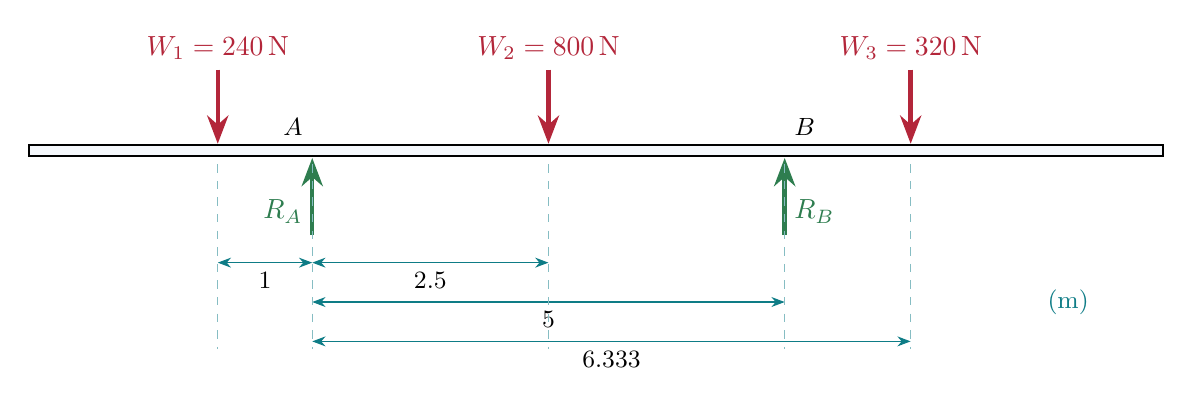
\begin{tikzpicture}[x=\u cm,y=1cm,>=Stealth]
  \draw[thick,fill=paper] (0,0) rectangle (12,0.14);
  % loads
  \foreach \x/\w/\lab in {2/240/W_1,5.5/800/W_2,9.3333/320/W_3}{
    \draw[->,line width=1.6pt,crimson] (\x,1.1) -- (\x,0.16);
    \node[above,crimson] at (\x,1.1) {$\lab=\w\N$};}
  % reactions
  \draw[->,line width=1.6pt,forest] (3,-1.0) -- (3,-0.02) ;
  \node[left,forest] at (3,-0.7) {$R_A$};
  \draw[->,line width=1.6pt,forest] (8,-1.0) -- (8,-0.02);
  \node[right,forest] at (8,-0.7) {$R_B$};
  \node[above left] at (3,0.14) {\small$A$};
  \node[above right] at (8,0.14) {\small$B$};
  % distances from A
  \draw[<->,teal] (2,-1.35) -- (3,-1.35) node[midway,below,text=black]{\small$1$};
  \draw[<->,teal] (3,-1.35) -- (5.5,-1.35) node[midway,below,text=black]{\small$2.5$};
  \draw[<->,teal] (3,-1.85) -- (8,-1.85) node[midway,below,text=black]{\small$5$};
  \draw[<->,teal] (3,-2.35) -- (9.3333,-2.35) node[midway,below,text=black]{\small$6.333$};
  \foreach \x in {2,3,5.5,8,9.3333} \draw[teal!50,dashed] (\x,-0.1) -- (\x,-2.45);
  \node[teal,font=\small] at (11,-1.85) {(m)};
\end{tikzpicture}
\end{center}

% =====================================================================
\section{សមីការលំនឹង}

\textbf{(ក) កម្លាំងផ្ដេក ៖} គ្មានបន្ទុកផ្ដេកទេ ដូច្នេះ
\[
  \sum F_x = 0 \;\Longrightarrow\; A_x = 0 .
\]

\textbf{(ខ) ម៉ូម៉ង់ធៀបនឹង $A$ ៖} (យកទិសច្រាសទ្រនិចនាឡិកាជាវិជ្ជមាន) ។
$W_1$ ស្ថិតនៅខាងឆ្វេង $A$ ដូច្នេះម៉ូម៉ង់របស់វាមានទិសច្រាសទ្រនិចនាឡិកា ៖
\[
  \sum M_A = 0:\qquad R_B(5) - 800(2.5) - 320(6.333) + 240(1) = 0
\]
\[
  5R_B = 2000 + 2026.67 - 240 = 3786.67
  \quad\Longrightarrow\quad
  {\color{crimson}\boxed{R_B = \tfrac{2272}{3} \approx 757.3\N\ \uparrow}}
\]

\textbf{(គ) កម្លាំងបញ្ឈរ ៖}
\[
  \sum F_y = 0:\qquad R_A + R_B - 240 - 800 - 320 = 0
  \quad\Longrightarrow\quad
  {\color{crimson}\boxed{R_A = \tfrac{1808}{3} \approx 602.7\N\ \uparrow}}
\]

\begin{checkbox}
យកម៉ូម៉ង់ធៀបនឹង $B$ វិញ (ទិសច្រាសទ្រនិចនាឡិកាជាវិជ្ជមាន) ៖
\[
  -5R_A + 240(6) + 800(2.5) - 320(1.333) = 0
  \;\Longrightarrow\; 5R_A = 3013.3
  \;\Longrightarrow\; R_A = 602.7\N \ \checkmark
\]
\end{checkbox}

\begin{note}
ចម្លើយ $R_A=624\N$ និង $R_B=736\N$ ដែលគេឃើញញឹកញាប់ មានផលបូកស្មើ $1360\N$ ដែរ
ប៉ុន្តែ\textbf{មិន}ផ្ទៀងផ្ទាត់ $\sum M_A=0$ ទេ ៖
$\;5(736)-3786.67=-106.7\ \mathrm{N\cdot m}\neq 0$ ។
កំហុសនេះកើតឡើងដោយដាក់ $W_3$ នៅចម្ងាយ $1\m$ ពី $B$ ជំនួសឲ្យ $\tfrac43\m$ ដែលត្រឹមត្រូវ ។
\end{note}

\begin{answer}
\[
  A_x = 0, \qquad
  R_A = \frac{1808}{3}\approx 602.7\N\ \uparrow, \qquad
  R_B = \frac{2272}{3}\approx 757.3\N\ \uparrow
\]
\end{answer}



\end{document}
